\documentclass[10pt]{extarticle}
\usepackage[letterpaper,margin=0.42in,top=0.36in,bottom=0.3in]{geometry}
\usepackage{fontspec}
\setmainfont{TeX Gyre Pagella}
\setsansfont{Arial}
\usepackage{xcolor,graphicx,booktabs,array,multicol,microtype,tikz,tcolorbox}
\usetikzlibrary{positioning,arrows.meta,calc}
\definecolor{ink}{HTML}{111827}
\definecolor{sec}{HTML}{5B6474}
\definecolor{blue}{HTML}{2563EB}
\definecolor{board}{HTML}{F6F7F9}
\definecolor{rule}{HTML}{CDD3DC}
\color{ink}
\pagestyle{empty}
\setlength{\parindent}{0pt}\setlength{\parskip}{2pt}
\linespread{1.0}
\setlength{\columnsep}{16pt}
\setlength{\columnseprule}{0.4pt}\def\columnseprulecolor{\color{rule}}
\newcommand{\sh}[1]{{\sffamily\bfseries\color{blue}\small\MakeUppercase{#1}}\par\vspace{1pt}}
\newcommand{\gl}[1]{{\color{sec}#1}}
\renewcommand{\arraystretch}{1.04}
\usepackage{ragged2e}\usepackage{enumitem}
\begin{document}
\RaggedRight
\fontsize{9}{10.8}\selectfont
% masthead
\begin{minipage}[b]{0.38\textwidth}
{\fontsize{31}{33}\selectfont\bfseries ICU Horizon}\\[1pt]
{\large\itshape\color{sec} From bench to bedside}
\end{minipage}\hfill
\begin{minipage}[b]{0.61\textwidth}\raggedleft\sffamily\fontsize{7.6}{9.4}\selectfont\color{sec}
\textbf{\color{ink}Team 7 \textperiodcentered{} CLIF} \textperiodcentered{} CIQ $\times$ NVIDIA $\times$ Lenovo Local AI Hackathon\\
Chicago, Nov 14--15, 2026\\
J.C. Rojas, MD, MS (Rush University) \textperiodcentered{} Kaveri Chhikara, MS (UChicago Medicine)\\
Vaishvik Chaudhari, MS (Rush University) \textperiodcentered{} Dema Therese, MS (UChicago Medicine)\\
Zewei (`Whiskey') Liao, MS (UChicago Medicine)
\end{minipage}

\vspace{2pt}{\color{ink}\rule{\textwidth}{1.1pt}}\vspace{3pt}

{\raggedright\fontsize{14.5}{17}\selectfont\bfseries Five 24-hour predictions for every patient in an intensive care unit (ICU), \color{blue}from a model we trained and run inside the hospital.\par}

\vspace{2pt}
\begin{multicols}{3}
\sh{The problem}
A small or rural ICU has a few life-support machines (ventilators, dialysis), no data-science team, and patient data that cannot leave the building. It learns it is short too late; help is a transfer hours away.

\columnbreak
\sh{What we built}
A bed board for the 07:00 team meeting: each patient's life support now, the probability of each event in the next 24 h, and unit totals against the machines on hand. An LLM chat answers questions about it.

\columnbreak
\sh{What is new for healthcare AI}
\begin{itemize}[leftmargin=8pt,itemsep=1pt,topsep=0pt,parsep=0pt,label={\color{blue}\textbullet}]
\item \textbf{A language model of health records:} pretrained from scratch on clinical-event tokens, not text.
\item \textbf{One pass, many outcomes:} linear probes on the last hidden state.
\item \textbf{Patient to unit:} probabilities sum into machine demand.
\item \textbf{On-prem:} trains and runs on the hospital's own hardware.
\end{itemize}
\end{multicols}

\vspace{2pt}
{\sffamily\bfseries\color{blue}\small THE FIVE PREDICTIONS\hfill\normalfont\itshape\color{sec} each is the chance it happens in the next 24 hours\par}\vspace{1pt}
{\sffamily\fontsize{8.6}{10.4}\selectfont
\begin{tabular*}{\textwidth}{@{\extracolsep{\fill}}lll@{}}
\toprule
\textbf{Prediction} & \textbf{Who plans for it} & \textbf{AUROC (95\% range)} \\
\midrule
Starts a ventilator {\color{sec}(a machine breathes for the patient)} & respiratory therapy & \textbf{0.78} (0.75--0.81) \\
Starts a vasopressor {\color{sec}(IV drug that raises blood pressure)} & pharmacy & \textbf{0.77} (0.74--0.80) \\
Starts CRRT {\color{sec}(a machine does the kidneys' work)} & ICU team & \textbf{0.88} (0.85--0.91) \\
Leaves the ICU {\color{sec}(to a lower-care ward, freeing the bed)} & bed manager & \textbf{0.80} ward \textperiodcentered{} \textbf{0.89} step-down \\
Dies {\color{sec}(a unit count, never shown on a bed)} & ICU team & \textbf{0.93} (0.91--0.95) \\
\bottomrule
\end{tabular*}}\\[1pt]
{\sffamily\fontsize{8}{9.6}\selectfont\color{sec}
Held-out test AUROC (patients never seen in training), 95\% bootstrap ranges. A patient already on a support gets no prediction for starting it.}

\vspace{5pt}
\begin{tcolorbox}[colback=board,colframe=blue,boxrule=0.9pt,arc=0pt,left=6pt,right=6pt,top=3pt,bottom=3pt,
 title={\sffamily\bfseries The model we trained, and the hidden layer},coltitle=white,colbacktitle=blue,fonttitle=\small,toptitle=1pt,bottomtitle=1pt]
\fontsize{8.7}{10.2}\selectfont\raggedright\hyphenpenalty=10000\exhyphenpenalty=10000
\begin{multicols}{2}
\textbf{1. Pretrain on health records.} A decoder-only transformer (layer design of NVIDIA Nemotron 3.5 Bolt E4B), 36.2M parameters, trained from scratch on both GB10s with DDP. Next-token objective plus a time-to-next-event loss. Vocabulary: 1,231 clinical-event tokens (lab and vital-sign values binned into ten levels, drugs, devices, transfers, time gaps); context 4,096 tokens.

\textbf{2. Embed each patient.} One forward pass over the patient's first 24 hours in the ICU. The last layer's hidden state at the final token, a \textbf{384-d vector}, is the patient embedding. No sampling, no generated futures.

\columnbreak
\textbf{3. Linear probes.} Six L2 logistic regressions on the embedding, fit once on training patients, output 24-hour event probabilities; leaving the ICU combines the ward and step-down probes. A new outcome is a new probe, not a new model. Probabilities sum into unit counts with an 80\% interval.

\textbf{4. LLM for explanation only.} NVIDIA Nemotron 3 Nano on vLLM answers questions by calling read-only tools on the forecast. It predicts nothing.
\end{multicols}
\end{tcolorbox}

\vspace{2pt}
{\sffamily\bfseries\color{blue}\small HOW WE USED THE CIQ STACK\hfill\normalfont\itshape\color{sec} the Fuzzball workflow on two local Lenovo ThinkStation PGX, one NVIDIA GB10 each\par}
\begin{center}
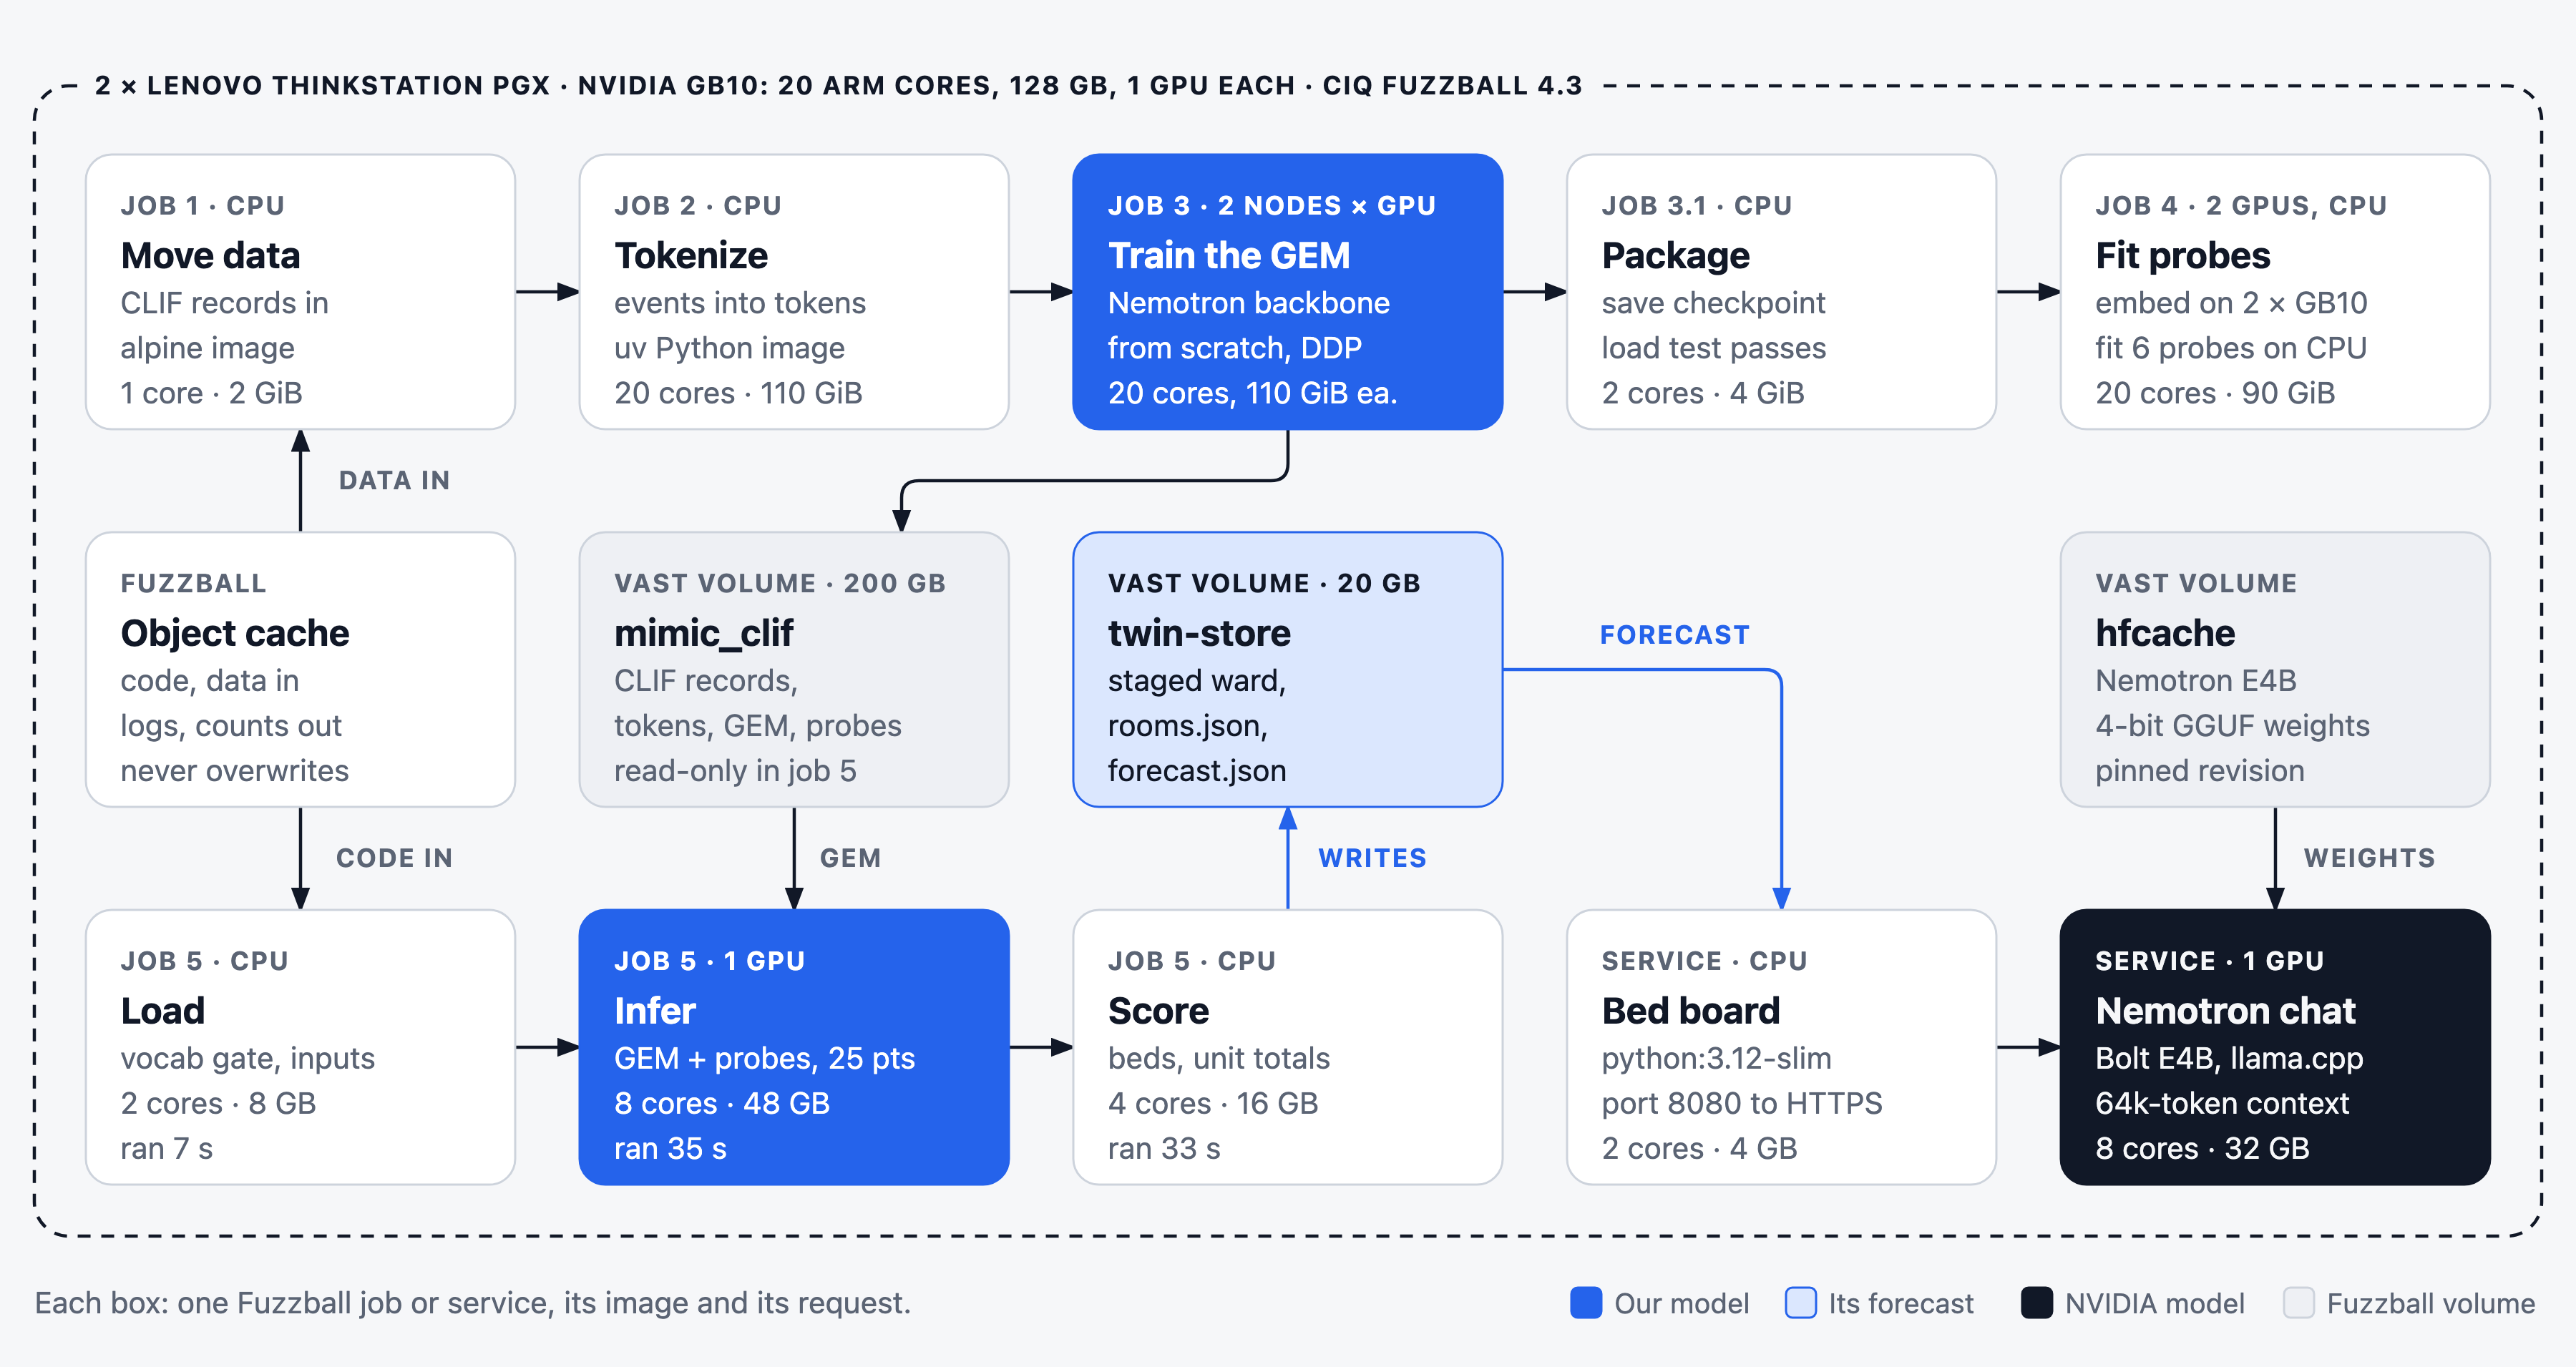
\includegraphics[width=0.76\linewidth]{../diagrams/architecture-print.png}
\end{center}
\vspace{-4pt}
{\sffamily\fontsize{8}{9.6}\selectfont\color{sec}
\textbf{\color{ink}Fuzzball:} Orchestrate schedules every job, container image and VAST volume; Substrate runs the NVIDIA containers (PyTorch, vLLM). We drove it with the Fuzzball MCP server and CLI. Code goes in and results come out only through the object cache. \textbf{\color{ink}All four tracks:} multi-node training (job 3 trains on both GB10s) \textperiodcentered{} inference (job 5 and Nemotron) \textperiodcentered{} scientific AI (a clinical model trained from scratch) \textperiodcentered{} cluster and scheduling (five workflows; inference frees its GPU before Nemotron starts).\par}

\vfill
{\color{ink}\rule{\textwidth}{0.9pt}}\\[2pt]
{\sffamily\fontsize{8}{9.6}\selectfont\color{sec}
\begin{minipage}[t]{0.74\textwidth}
Code: \textbf{\color{ink}github.com/vaishvikc/ICU-Twin}\\ A research prototype built on past, de-identified ICU records. Not a medical device.
\end{minipage}\hfill
\begin{minipage}[t]{0.25\textwidth}\raggedleft{\normalsize\bfseries\color{ink}\rmfamily Nothing leaves the building.}\end{minipage}}
\end{document}
